%%Put forth research questions, which will be answered in Conclusions
%%State why this problem was chosen based on weaknesses that existed in mid surface generation
%%Motivation for the choice of the research question has to be given. This motivation must be based on/linked with the following issues as well.
%%Motivate the problem and state your hypothesis 
%%	Tell a story, and tell it well
%%	Use plenty of concrete examples (or a running example) and figures 
%%	Quote data sources, e.g., industry analysts, market surveys, case studies 
%%	People often (and naturally) make up their mind within the first few pages
%%	Introduce all your terminology here – especially, acronyms you plan to use often
%%Do ……
%%	Provide a concrete problem definition, accessible to a computer-literate person, without “dumbing down” the problem to people in your field
%%	Provide a concrete list of your thesis’ contributions  
%%Don’t ….. 
%%	Oversell your thesis or its claims – be honest and you will be respected
%%	Use hyperbole (e.g., “highly reliable”, “extremely efficient”)
%%	Try to confuse the reader with big words – plain, simple English is best
%%	Try to sound like your thesis covers your entire field (unless it does, of course!) 


\section{Introduction}

\todo{Telephone comment: Change the beginning of this paragraph, we don't want direct CAE reference but a start with some global manufacturing, product context. [DONE]}

These days, industries worldwide are facing several challenges due to stiff global competition. These include rapid changes in the customer preferences, shorter products lives, continuous changes due to disruptive innovations, frequent design changes, etc., forcing industries to get their products in the market, quickly. Time needed from conceptualization of the product till delivering it in market, is known as ``Time to Market''. Thus, goal of the industries is to shorten the Time to Market by making Product Development Process (PDP) more efficient. 

	\bigskip
	
	\begin{figure} [!h]
		\centering
		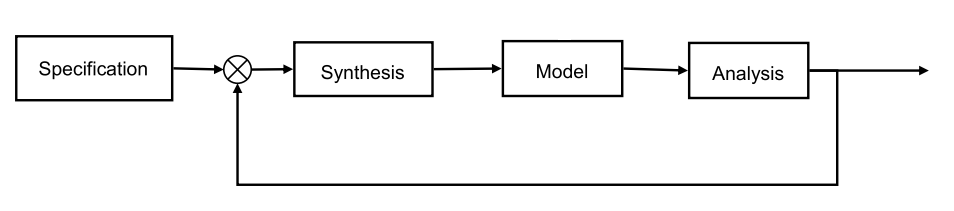
\includegraphics[width=0.9\linewidth]{..//Common/images/PDPProcess.png}
		\caption{Product Development Process (PDP) (Source: Stolt\cite{Stolt2008})}
		\label{fig:introduction:PDPProcess}
	\end{figure}
	
	\bigskip
	
Figure \ref{fig:introduction:PDPProcess} shows stages of PDP as presented by Stolt\cite{Stolt2008}. It starts with ``Specification'' stage where the product requirements are studied, prioritized and are turned into concrete specifications. At ``Synthesis'' stage, various alternatives to address the specifications are evaluated. The most satisfactory alternative is designed at ``Model'' stage. Finally the designed model is evaluated against the specifications at the `'Analysis'' stage. If the analysis results are not satisfactory, then the process is iterated from ``Synthesis'' stage again, until a satisfactory product is arrived at.

PDP can be made more efficient either by reducing number of iterations or by reducing the time needed for each iteration, i.e. the time needed for the design and analysis of the product.
In past, before advent of computers, the design used to get done by manual calculations, sketches, etc., whereas the analysis was performed by testing physical prototypes of the product. In modern times, Computer-aided Design (CAD) applications are used extensively for design, whereas Computer-aided Engineering (CAE) applications are used for testing \& simulation of the products, virtually. Design calculations provide shape and size of the product. These shapes are modeled in CAD using various operations, such as extruding a sketch, revolve, fillet, etc. These modeling operations are known as features. The resultant CAD models are used for various downstream applications such as Computer-aided Manufacturing (CAM), visualizations, CAE, etc. In CAE, a CAD model is analyzed by decomposing it into mesh of elements, applying loads and boundary conditions and then solving the mesh for parameters such as stress, strain, displacements, etc. Thus, CAD-CAE process is a core stage of the modern PDP process and making it more efficient is key to reduce the Time to Market.

%
%Evolution of the PDP can be broadly classified into two eras, the pre-computers era and the computer era.  In the pre-computers era, calculations were done on paper, and prototypes were tested physically. This process was iterated till the design was satisfactory. 
%
%In the computer era, the PDP also goes through similar iterations, but the difference is that many of its sub-processes are handled with the help of computers. With increasing availability of vast and cheaper computational power, it has become imperative to leverage it for the core of PDP i.e. Design-Analysis, via approaches known as Computer-aided Design(CAD) and Computer-aided Engineering(CAE). Computers help in getting product design(CAD)  and its virtual validation(CAE), not just faster, but allow much needed iterations in far lesser costs than the physical counterparts. 

\section{CAD-CAE Process} \label{sec:intro:cadcae}

\todo{Review comments: Change this subsection to section. Either give complete description of CAD-CAE and to end process ow within this section add subsections pertaining to different steps in CAD-CAE product design cycle. [DONE]}

One of the critical aspect of the CAD-CAE process is the transformation of CAD model to CAE model. CAD models are often highly detailed, as they need to have information needed by various downstream applications. For CAE, many such details are not needed, which add to the complexities in mesh generation and demand more computational power-time, for analysis. Removing such details and simplifying the CAD model is a necessary transformation and is a significant portion of preprocessing done to prepare the CAE model. This simplification process, is often not automatic and straightforward, but is time consuming, manual and tedious.
%CAE offers virtual analysis of the product without building any physical prototype.  Even though the result fidelities are usually not as satisfying as the physical  prototyping experiments, CAE analysis is quick and often cost effective validation method. It helps designers understand the physical behaviors of the product, evaluate alternatives, perform experiments, do iterations and make decisions before committing the designed products to manufacturing.   So, although CAE does not fully \replaced{avoid }{takeaway} the necessity to build the physical models, but it can vastly reduce their number of iterations, thereby saving the cost and time. Due to such substantial advantages, industry \replaced{strongly needs }{desires nothing less than } a fully automated and reliable analysis process, but the current CAE systems are far from achieving this goal. The main reason is the presence of  different purposes of CAD-CAE data. CAD models are far more detailed than what is needed by CAE. This transformation from CAD model to CAE model is often manual and tedious process. 
\replaced{These problems can be addressed by a robust and automated simplification in the CAD-CAE process}{To alleviate these lacunae, D. H. Brown Associate report   claims that  the system that would possibly do robust and automated CAD-CAE process would incorporate feature information to create more intelligent analysis models}\cite{Halpern1997}. 
%CAD model, as mentioned before, being a generic input to various downstream applications, typically contains lots of details, some of which are irrelevant to CAE.  The unnecessary details add to the complexities in mesh generation, and demand more computational power-time for a relatively smaller gain in the accuracy of the results\cite{Thakur2009}. Also, the complex models may often lead to ill-conditioned matrices and hence working with non-simplified complex models may produce inaccurate results\cite{Saad2003}. Hence, simply utilizing more powerful computers will not solve the problem associated with the highly complex models. CAD models are, thus, simplified before sending them to CAE analysis. This transformation is known as ``Model Simplification''.  Although the Model Simplification significantly improves the analysis time, the deviation from the original shape, does introduce some error. Whenever, the gain in computation outweighs the error, model simplification is used. 


	\bigskip
	
	\begin{figure} [!h]
		\centering
		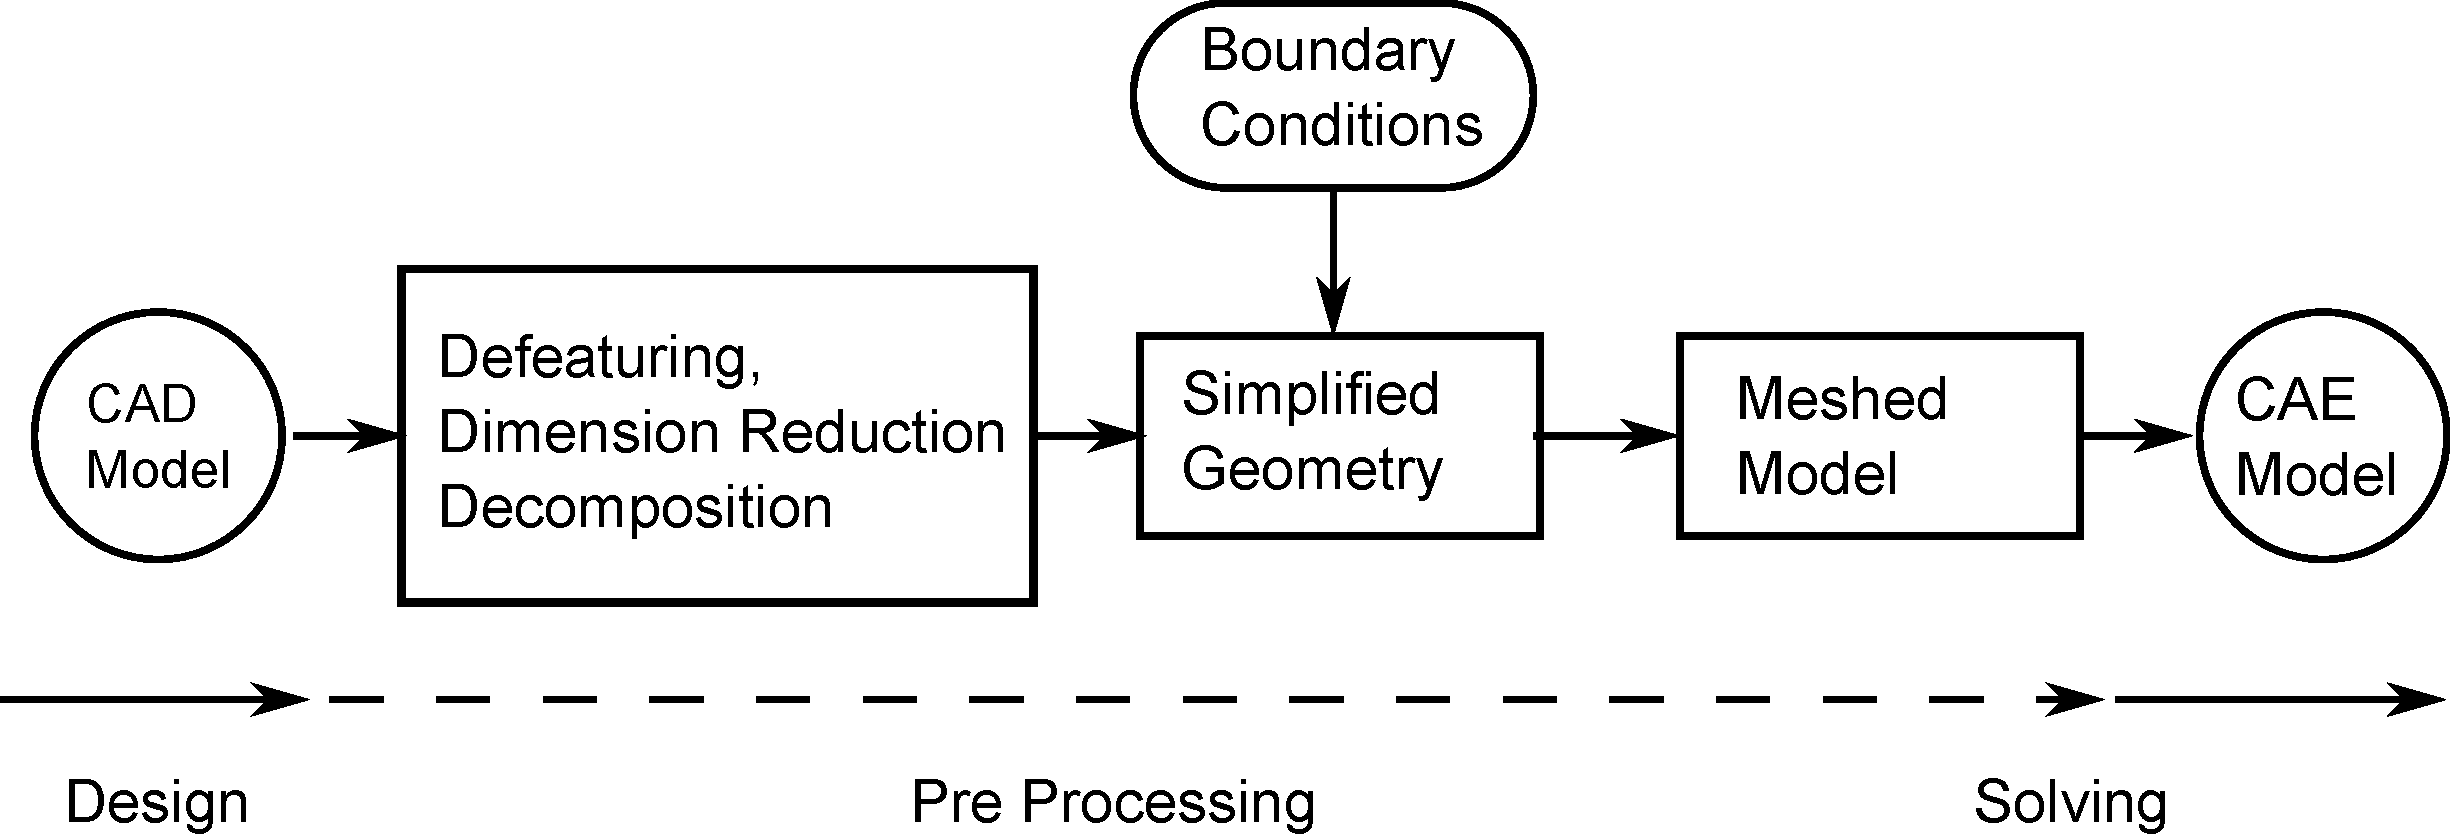
\includegraphics[width=0.9\linewidth]{..//Common/images/CADCAEGeneralProcess.pdf}
		\caption{Computer-aided PDP (Source: Tierney\cite{Tierney2013})}
		\label{fig:introduction:cadcaeworkflow}
	\end{figure}


	\bigskip
	
\todo{Review comment: Do not quote too many references here but provide a very high level overview of CAD CAE process. [REMOVED CITATIONS. REARRANGED]}

Figure \ref{fig:introduction:cadcaeworkflow} shows various stages which a CAD model undergoes to be ready for CAE analysis. Simplification, as shown in the first box, mainly consists of defeaturing and dimensions reduction. In defeaturing, irrelevant details are removed by removing corresponding features. Due to defeaturing, meshing is not unnecessarily dense and complicated around the irrelevant details. Thus defeatured model reduces number of elements, which correspond to lesser degrees of freedom (DoFs) of the mesh, thereby saving analysis time and resources substantially.  In dimension-reduction, shapes like slender-bar, thin-wall are transformed into their lower dimension representations such as curves, surfaces, respectively. Lower dimension representations are used for lower dimension element types such as beams or shell which have far lesser DoFs than the solid elements. Thus use of dimension reduction reduces analysis time and resources further.
% Once meshing is complete, loads and boundary conditions are applied. Based on the analysis type (static, dynamic, modal) further computations are carried out. Output results are presented either in the form of reports or visualizations. If this analysis finds certain weaknesses, design changes are suggested, which, when done, the analysis iteration is carried out once more. This process repeats till satisfactory model is arrived at.

Dimension reduction transformation is widely used in CAE analysis of thin-walled parts, such as sheet metal and plastic products.  CAD models of these parts are transformed into a representative surface known as ``Midsurface''. It is a surface lying midway of a thin-walled CAD model and mimicking its shape.  Getting a correct midsurface is critical to CAE analysis of thin-walled parts.
%
%For sheet-metal, plastic products (generically classified as `thin-walled'),  a quick and fairly accurate CAE analysis is possible by idealizing their CAD solid models to the equivalent surface representation called ``Midsurface'' (Note: `Midsurface', `Mid-plane' and  `Medial Object' are used synonymously in this work, unless specified otherwise). It can be envisaged as a surface lying midway of a thin-walled solid, and mimicking its shape.
%Despite an extensive research and high commercial demand, there is still a significant disconnect is observed between CAD and CAE. It is mainly due to lack of automated, robust defeaturing and dimension-reduction approaches\cite{Nolan2015}.  The present research focuses on the dimension-reduction by developing an automatic, deterministic and generic approach for the computation of a well-connected midsurface, along with associated defeaturing, for thin-walled CAD models.
	
\section{Midsurface for CAE Analysis of Thin-walled Parts} \label{sec:intro:cadcae}

CAE analysis of the thin-walled parts using 3D solid mesh elements such a Hexahedral or Tetrahedral, is expensive in terms of computing resources and time taken. 2D surface mesh elements such as Shell, are preferred as they give reasonably accurate analysis results, while requiring far lesser computational resources and time~\cite{Elangovan2012}.  Shell elements need midsurface and thickness values for their definition and usage. Thus, midsurface is the most widely used representation of thin-walled parts for CAE analysis.
 
 Most midsurface generation approaches are based on the final shape of the CAD model. It is typically represented by a data structure known as Boundary Representation (Brep). In Brep, a solid shape is represented by a set of connected faces to form a closed volume. Midsurface is computed either by applying geometric transformations or by using heuristic rules on Brep. 
 
Face pairing is one of the most popular midsurface computation method based on Brep. Faces opposite each other are detected to form face-pairs. Each face pair computes an equidistant surface in the middle, called midsurface patch. These patches are then, either extended or trimmed to join at a common edge to form a well-connected midsurface. Although this approach works well on simple, academic models, it often fails in case of real-life, complex models. Failures are in the form of gaps between patches, overlaps, midsurface not lying midway, etc.  Thus, minimizing the failures and devising a robust approach to compute a well-connected midsurface is critical to the CAD-CAE process of thin-walled parts.
 
% In complex Brep shapes it is challenging to find appropriate face pairs and to join midsurface patches correctly. Instead of the final Brep shape, few approaches use the model construction information, in the form of features, to compute the midsurface~\cite{Robinson2006}. This feature-based approach is promising as at each feature step in the construction, shapes are relatively simpler than the final model shape.
% 
% So, they do not leverage feature information available in modern feature based CAD applications. The reasons are multi-fold.  Since beginning, CAD and CAE products evolved separately, by different companies. Interoperability between them was through neutral B-rep formats. It was done so for avoiding export of  proprietary design intent information in the form of features. 
% \deleted{Now, with far more integrated CAD-CAE environments, and access of features through APIs it is possible to leverage feature-information in CAE, as demonstrated in the present research for generating midsurface.} 
% 
% In recent times, CAD systems have started exposing the feature information through Application Programming Interfaces (API) for better support to 3rd party applications. Now it is possible to build own algorithms, as this research does, leveraging the feature information as it is a  rich source of part creation information. It can have advantages over current 
%midsurface generation algorithms, which are largely based on rudimentary heuristics and lack appropriate topological validation. The work presented in this thesis aims at effectively utilizing feature information for simplification of model as well as the feature tree so that the part model can be represented by a very minimal set of features and complexity of midsurface generation problem is drastically reduced. Further midsurface connections are resolved by a very generic algorithms that cover a wide range of connectivity problems. The research further adds apt topological validation to correlate CAD part model and corresponding midsurface.

\todo{Review comment: I don't think this type of citation (footnotes) fits into specified format. [REMOVED FOOTNOTES]}
\todo{Review comment: You only finished till simplification what are the further steps till CAE analysis is done and how that info is used? [ADDED NOTES FOR FURTHER CAE STEPS]}
\todo{Review comment: Once you have introduced term midsurface in CAD CAE process, no need to define it here. Only talk about why midsurface are still critical for thin walled parts. [DONE]}
\todo{Review comment: Change heading of this paragraph. [DONE. MOVED SANDIA REPORT PARA TO PREVIOUS SECTION]}	
\todo{[ADDED FOLLOWING PARAGRAPH AS PER SUGGESTION. NOT USED `MIDCURVE' AS NOT DEFINED SO FAR]} 

\section{Motivation of Research}

 Midsurface is the most suitable representation for the CAE analysis of thin-walled parts' CAD models. 
 A Sandia report~\cite{Ming2012} states that, for the complex engineering models, their simplification amounts to about 60\% of the overall analysis time, whereas the mesh generation consumes about 20\% and solving the actual problem takes about 20\%.  In the shipping industry, more than 80\% of CAE engineer's time is spent on modeling dimensionally reduced entities\cite{Austreng2007}. Automex\cite{Automex} observed that the complexity involved in generating midsurfaces takes about 70 to 90\% of the pre-processing time. % In case of crash simulation components, this time can go up to 14 days.
Thus,  computing well-connected midsurface is highly critical to the industry.

%So, even in this age of scalable and near-infinite computing power, it is still desirable to have  this idealized representation, instead of just pouring millions of 3D elements\cite{Abbey2013}. With far lesser nodes and degrees of freedom one is able to run more design iterations quickly.  Thus, midsurface is the most suitable idealization for the analysis of thin-walled parts.   Because of this  advantage,  having an automatic, deterministic and generic method for computing well-connected midsurface is critical to the  industry.
Despite extensive research, many midsurface computation approaches fail to generate a well-connected midsurface, especially for the complex part shapes. Correcting the errors is mostly a manual, tedious and highly time-consuming task, requiring hours to days. This correction time can be nearly equivalent to the time it can take to create the midsurface manually from scratch\cite{Stolt2006}. 

Thus, the present research is primarily concerned with the design and implementation of a system to generate a well-connected midsurface for thin-walled parts.

\section{Scope of the Work}  \label{sec:litsurvey:rscope}

\todo{TODO: RE-CHECK THE MEANING OF THE PARAGRAPH}

%% As explained in Section \ref{sec:intro:cadcae}, modern PDP process heavily depends on CAE for validation of the CAD models. Validation is for assessing strength, studying interaction with fluids, checking abilities to withstand heat-temperature, understanding model behavior, etc.  

Thin-walled parts are present in a variety of domains, such as plastics, sheet metal, machined components, etc. They are either constant thickness parts such as in sheet metal domain, or variable thickness parts, as in plastics domain.  D W Brown Report~\cite{Halpern1997} suggests that sheet metal parts is one of the most widely used sub-category, with approximately 40\% share amongst the manufacturing processes. They are found in a wide variety of applications such automobile, aircraft, shipbuilding, consumer products, electronic equipments, etc.  


\bigskip

\def \myfigstairspcolumnwidth{0.21}

\begin{figure}[h!]
\centering  
\subfloat[Harvester]{\label{fig:introduction:harvester}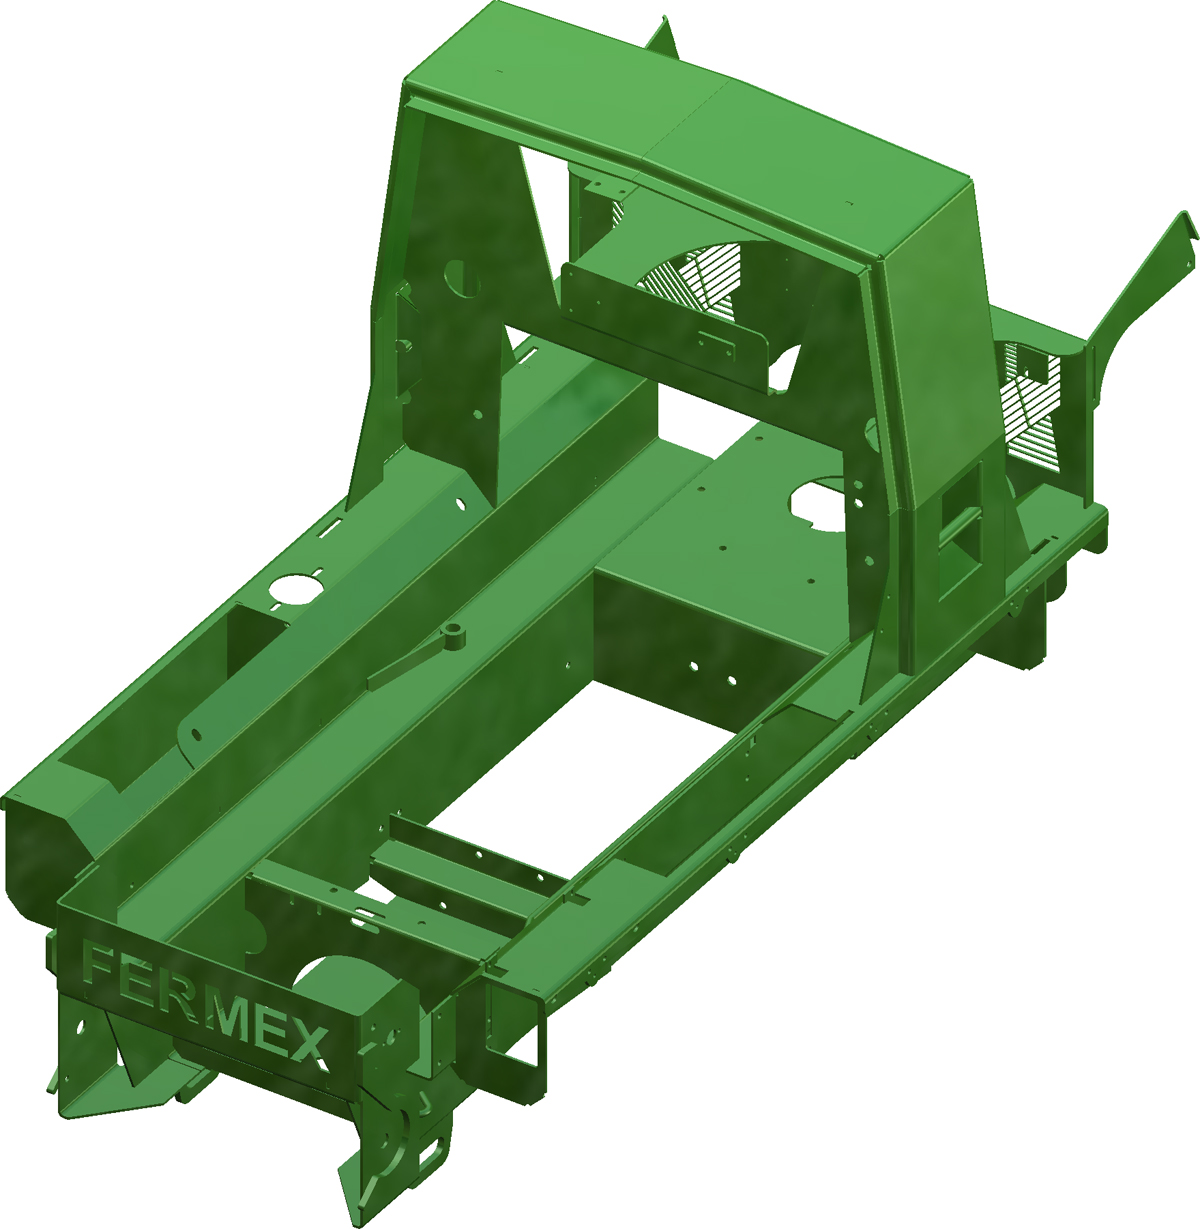
\includegraphics[width=0.16\linewidth]{../Common/images/SheetMetal_isd_cad_blech_vermeer}} \quad
\subfloat[Enclosure]{\label{fig:introduction:enclosure}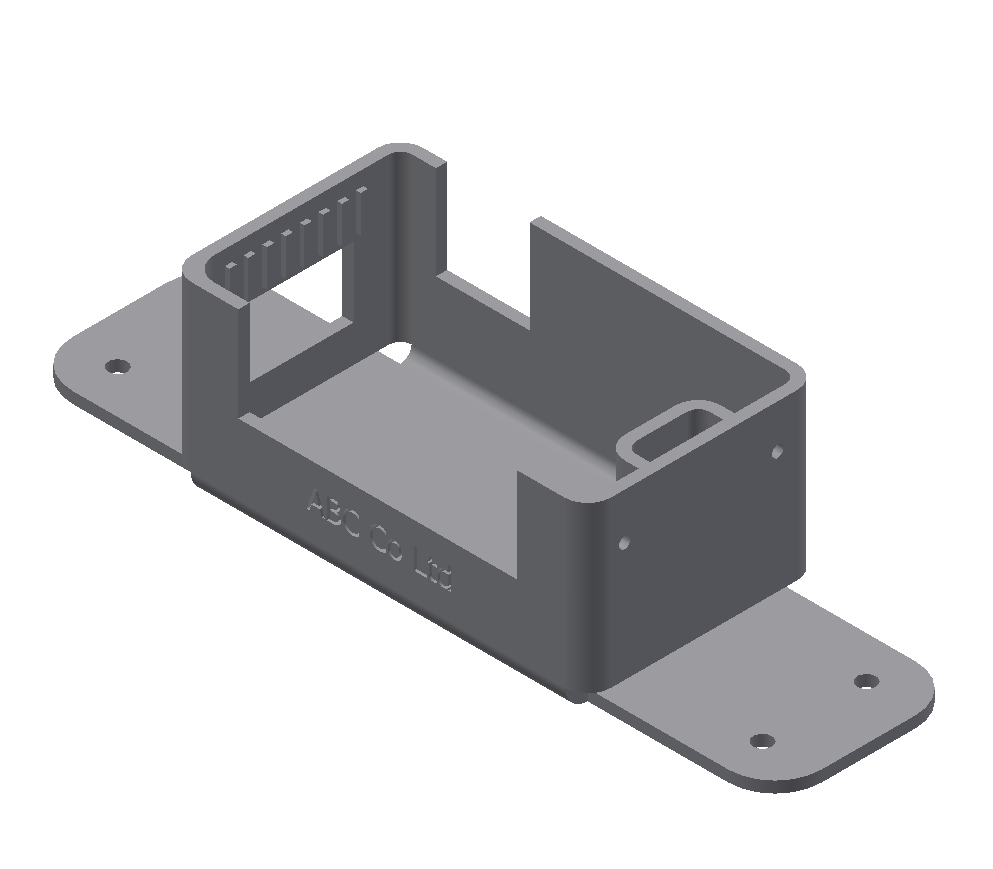
\includegraphics[width=\myfigstairspcolumnwidth\linewidth]{../Common/images/SheetMetal_Medium_Enclosure_OriginalPart}} \quad
\subfloat[Bracket]{\label{fig:introduction:bracket}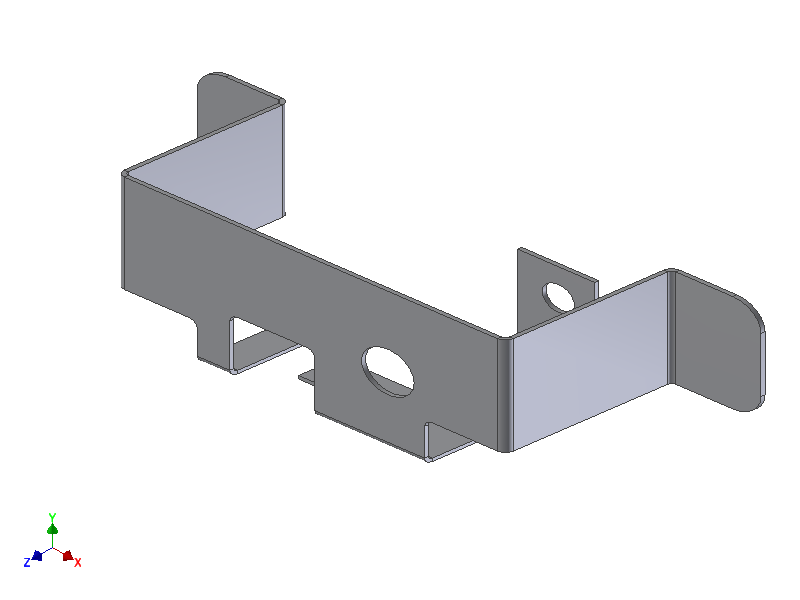
\includegraphics[width=\myfigstairspcolumnwidth\linewidth]{../Common/images/SheetMetal_Simple_UBracket_OriginalPart}}   \quad
\subfloat[Duct]{\label{fig:introduction:duct}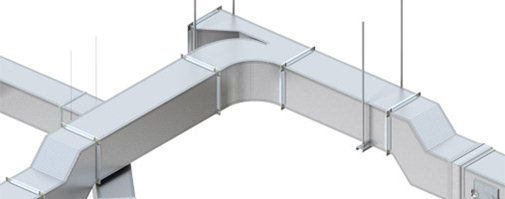
\includegraphics[width=\myfigstairspcolumnwidth\linewidth]{../Common/images/SheetMetal_KDuct-Main-Render}}
\caption{Variety of Sheet Metal Parts}
\label{fig:introduction:sheetmetalsamples}
\end{figure}


\bigskip

\todo{Review comment: Can computer casing be replaced by one of the case study parts? Use stapler part. [DONE]}

Figure \ref{fig:introduction:sheetmetalsamples} shows some of the sheet metal parts, such as an agricultural harvester frame~\cite{harvester}, an enclosure commonly used in electrical systems, a bracket found in mechanical systems and HVAC ducting. Looking at the range of the sheet metal products, any improvement in their CAE analysis will have a significant impact on the product development process of all these domains. \replaced{Hence the domain of sheet metal parts is being considered in the proposed research. }{So, the present research plans to focus on getting the most crucial sub-process of the CAE prepossessing right, i.e. generating a better midsurface.}

Thus, the present research work focuses on proposing an approach to generate a well connected midsurface, which will improve results of CAE analysis of sheet metal CAD models. The approach is elaborated in details in the following chapters of this thesis.

\section{Organization of the Thesis}

The subsequent organization of the thesis is as follows:

\begin{itemize}[label={},leftmargin=*]

\item Chapter  \ref{ch:Survey} reviews the relevant literature on the traditional midsurface generation approaches along with auxiliary approaches such as defeaturing and decomposition. Specific issues and limitations of these approaches are highlighted. The chapter concludes by outlining objectives of the present research work.

\item Chapter \ref{ch:Proposal} presents an overview of the proposed system to generate well-connected midsurface of sheet metal feature based CAD model. It describes major modules involved with respect to their functional capabilities and interrelationships.

\item Chapter \ref{ch:Defeaturing} presents at length the algorithms for defeaturing.  It initially outlines the phases and then subsequently presents in details the methodology and the algorithms to generate the simplified feature based CAD model.

\item Chapter \ref{ch:Abstraction} presents the algorithms to transform the sheet metal features to a generalized finite set of features. Such generalized feature based model aids in reducing the complexity of the algorithms.

\item Chapter \ref{ch:Midsurface} \replaced{details out various strategies to generate midcurves, midsurface patches and dedicated algorithms to join them.}{reports at length various steps the abstracted model goes through, such as cellular decomposition, midsurface patch generation, patch joining, etc. Towards the end of this chapter, various characteristic shapes are used to demonstrated the efficacy of the algorithms.}

\item Chapter \ref{ch:Validation} presents a newly proposed methodology for validating midsurface based on topological considerations.

\item Chapter \ref{ch:Testing} demonstrates the capabilities of the proposed system for generating quality midsurface with reference to typical model case studies.

\item Chapter \ref{ch:Conclusions} summarizes the research work highlighting the major contributions and outlines direction of the future work.
\end{itemize}



